% lecture07.tex: Lecture 7: Planetary Surfaces, Geology, Geomorphology, & Geophysics
% Planetary Systems, Kapteyn Institute

\documentclass[aspectratio=169, 11pt]{beamer}

% ── Theme and macros ────────────────────────────────────────
\usepackage{../common/beamerthemeIPS}
% macros.tex: Shared math macros for IPS lecture slides
% Mirrors definitions in book/_config.yml for consistency
% Uses \providecommand to avoid conflicts with unicode-math

% ── Derivatives ─────────────────────────────────────────────
\providecommand{\dv}[2]{\frac{\mathrm{d} #1}{\mathrm{d} #2}}
\providecommand{\dd}{}\renewcommand{\dd}{\mathrm{d}}
\providecommand{\pdv}[2]{\frac{\partial #1}{\partial #2}}

% ── Solar quantities ────────────────────────────────────────
\newcommand{\Msun}{M_{\odot}}
\newcommand{\Rsun}{R_{\odot}}
\newcommand{\Lsun}{L_{\odot}}

% ── Planetary quantities ────────────────────────────────────
\newcommand{\Mearth}{M_{\oplus}}
\newcommand{\Rearth}{R_{\oplus}}
\newcommand{\Mjup}{M_{\mathrm{J}}}
\newcommand{\Rjup}{R_{\mathrm{J}}}

% ── Constants ───────────────────────────────────────────────
\newcommand{\kB}{k_{\mathrm{B}}}

% ── Media links ─────────────────────────────────────────────
% Clickable button that opens the animated or video version of a
% figure, e.g. \mediabutton{https://...gif}{Play animation}
\providecommand{\mediabutton}[2]{\href{#1}{\beamergotobutton{#2}}}

\graphicspath{{figures/}{../common/}{../../book/07_surfaces/figures/}}

% ── Metadata ────────────────────────────────────────────────
\title[Lecture 7: Surfaces]{Lecture 7: Planetary Surfaces\\Geology, Geomorphology, \& Geophysics}
\subtitle{Planetary Systems}
\author[L7]{Tim Lichtenberg}
\institute{Kapteyn Astronomical Institute\\University of Groningen}
\date{2026}
\titlebgcredit{Olympus Mons, Mars. Credit: NASA/JPL/USGS}

% ════════════════════════════════════════════════════════════
\begin{document}

% ── Title slide ─────────────────────────────────────────────
\begin{frame}[plain,noframenumbering]
  \titlepage
\end{frame}

% ── Learning objectives ─────────────────────────────────────
\begin{frame}{Learning objectives}
  By the end of this lecture, you will be able to:
  \vskip8pt
  \begin{itemize}
    \item Distinguish endogenic and exogenic surface processes
    \item Describe the three stages of impact crater formation
    \item Derive the crater scaling law $D \sim (E/\rho g)^{1/4}$ from dimensional analysis
    \item Use crater counting to determine relative and absolute surface ages
    \item Compare volcanic, tectonic, and erosional styles across the solar system
  \end{itemize}
\end{frame}

% ── Recap ───────────────────────────────────────────────────
\begin{frame}{Recap: Lectures 5 \& 6}
  \begin{itemize}
    \item Hydrostatic equilibrium and the scale height set an atmosphere's structure
    \item Greenhouse warming: $T_s > T_{\mathrm{eff}}$; Clausius-Clapeyron sets where clouds form
    \item The carbonate-silicate cycle is Earth's long-term thermostat
  \end{itemize}
  \vskip8pt
  \textbf{Today:} What shapes the \textit{surfaces} of planets and moons?
\end{frame}


% ════════════════════════════════════════════════════════════
\sectionimage{surface_processes_montage}{Valles Marineris hemisphere of Mars, Viking Orbiter mosaic. Credit: NASA/JPL/USGS}
\section{Surface processes}
% ════════════════════════════════════════════════════════════

% ── Endogenic vs exogenic ─────────────────────────────────
\begin{frame}{Endogenic vs.\ exogenic processes}
  A surface is a geological record: processes that build landforms compete with processes that destroy them.
  \vskip8pt
  \begin{columns}[T]
    \column{0.48\textwidth}
    \textbf{Endogenic} (internal heat):
    \begin{itemize}
      \item Volcanism
      \item Tectonics (faulting, folding)
    \end{itemize}

    \column{0.48\textwidth}
    \textbf{Exogenic} (external forces):
    \begin{itemize}
      \item Impact cratering
      \item Erosion (wind, water, ice)
    \end{itemize}
  \end{columns}
  \vskip8pt
  \keyresult{Hot interior: endogenic processes win. Dead interior: the surface keeps its ancient craters.}
\end{frame}

% ── Dominant processes table ──────────────────────────────
\begin{frame}{Dominant surface process by body}
  \centering
  \small
  \begin{tabular}{l c c}
    \toprule
    \textbf{Body} & \textbf{Dominant process} & \textbf{Key evidence} \\
    \midrule
    Moon   & Impact cratering & Saturated highland craters, $>$4~Gyr \\
    Earth  & Plate tectonics + erosion & Ocean floors $<$200~Myr; rapid weathering \\
    Mars   & Volcanism + impacts & Olympus Mons; cratered southern highlands \\
    Venus  & Volcanism & Volcanic plains cover $\sim$80\% of surface \\
    Io     & Tidal volcanism & $\sim$300--400 active volcanoes; age $<$1~Myr \\
    Europa & Ice tectonics & Lineae, chaos terrain, very few craters \\
    \bottomrule
  \end{tabular}
\end{frame}


% ════════════════════════════════════════════════════════════
\sectionimage{crater_morphology}{Lunar crater morphology. Credit: NASA/GSFC/ASU}
\section{Impact cratering}
% ════════════════════════════════════════════════════════════

% ── Universality ──────────────────────────────────────────
\begin{frame}{The most universal geological process}
  \begin{itemize}
    \item \textbf{Every} solid body in the solar system bears impact craters
    \item Without atmosphere or geology (Moon, Mercury), craters survive billions of years
    \item Impact velocities 10--70~km\,s$^{-1}$, set by orbital mechanics (Lecture~2)
  \end{itemize}
  \vskip8pt
  \keyresult{A 1~km rocky asteroid at 20~km\,s$^{-1}$ carries $E_k = \tfrac{1}{2}mv^2 \approx 3 \times 10^{20}$~J, about 1000 times the largest nuclear weapon, released in under a second.}
\end{frame}

% ── Three stages ──────────────────────────────────────────
\begin{frame}{Three stages of crater formation}
  \begin{columns}[T]
    \column{0.32\textwidth}
    \textbf{1. Contact and compression}
    \begin{itemize}
      \item Shock wave into target and impactor
      \item $\sim$100~GPa; melting and vaporisation
      \item Over in $<1$~s
    \end{itemize}

    \column{0.32\textwidth}
    \textbf{2. Excavation}
    \begin{itemize}
      \item Rarefaction wave throws material out
      \item Transient cavity, depth:diameter $\approx$ 1:3
      \item Ejecta blanket around the rim
    \end{itemize}

    \column{0.32\textwidth}
    \textbf{3. Modification}
    \begin{itemize}
      \item Cavity collapses under gravity
      \item Small: walls slump, \textbf{simple crater}
      \item Large: floor rebounds, \textbf{central peak}
    \end{itemize}
  \end{columns}
\end{frame}


% ════════════════════════════════════════════════════════════
\sectionimage{mercury_caloris_basin}{Caloris basin, Mercury. Credit: NASA/Johns Hopkins APL/Carnegie Institution of Washington}
\section{Blackboard derivation: the crater scaling law}
% ════════════════════════════════════════════════════════════

% ── Setup ─────────────────────────────────────────────────
\begin{frame}{Setup: crater size from dimensional analysis}
  \textbf{Goal:} How does crater diameter $D$ depend on impact energy $E$, target density $\rho$, and surface gravity $g$?
  \vskip10pt
  In the \textbf{gravity regime} (craters $\gtrsim$100~m, where gravity limits size):
  $$D = C \, E^a \, \rho^b \, g^c$$
  \vskip6pt
  Dimensions ($M$, $L$, $T$):
  \vskip4pt
  \begin{tabular}{l l}
    $[D]$ & $= L$ \\
    $[E]$ & $= M L^2 T^{-2}$ \\
    $[\rho]$ & $= M L^{-3}$ \\
    $[g]$ & $= L T^{-2}$ \\
  \end{tabular}
  \vskip8pt
  \textit{To the board.}
\end{frame}

% ── Strength vs gravity regime ────────────────────────────
\begin{frame}
  \centering
  \makebox[\linewidth][c]{\includegraphics[width=0.95\paperwidth, height=0.80\paperheight, keepaspectratio]{holsapple1993_strength_gravity_regimes}}\\
  {\footnotesize The two cratering regimes for a target with strength, at impact velocities $U = 2.5$, 10 and 40~km\,s$^{-1}$. Reproduced from Holsapple (1993), Fig.~3.}
\end{frame}

% ── Result and its range ──────────────────────────────────
\begin{frame}{Where the fourth-root law applies}
  \begin{columns}[c]
    \column{\recapfigcol}
    \ipsrecapfig{holsapple1993_strength_gravity_regimes}
    \source{Holsapple (1993), Fig.~3}

    \column{\recaptextcol}
    \footnotesize
    \keyresult{$D \sim (E/\rho g)^{1/4}$: doubling $E$ grows $D$ by only $2^{1/4} \approx 1.19$}
    \vskip2pt
    \begin{itemize}
      \item \textbf{Left, strength regime:} cohesion limits growth, curves separate
      \item \textbf{Right, gravity regime:} one law; planetary craters live here; below $\sim$100~m on the Moon the law fails
      \item At fixed $v$ and $\rho$: $E \propto L^3$, so $D \propto L^{3/4}$ (1~km impactor, 16.5~km crater)
    \end{itemize}
  \end{columns}
\end{frame}


% ════════════════════════════════════════════════════════════
\sectionimage{crater_counting}{Lunar farside. Credit: NASA/GSFC/ASU}
\section{Crater morphology and chronology}
% ════════════════════════════════════════════════════════════

% ── Morphological classes ─────────────────────────────────
\begin{frame}{Crater morphology: three classes}
  \begin{columns}[c]
    \column{\recapfigcol}
    \ipsrecapfig{crater_morphology}
    \source{NASA/GSFC/ASU}

    \column{\recaptextcol}
    \small
    \begin{enumerate}
      \item \textbf{Simple} ($D < D_t$)\\
      Bowl-shaped; depth:diameter $\approx$ 1:5\\
      Moon: $D_t \approx 15$~km
      \vskip4pt
      \item \textbf{Complex} ($D_t < D \lesssim 300$~km)\\
      Central peak, terraced walls, flat floor: gravity overcomes wall strength
      \vskip4pt
      \item \textbf{Multi-ring basins} ($D \gtrsim 300$~km)\\
      Orientale (930~km), Caloris (1550~km), Hellas (2300~km)
    \end{enumerate}
  \end{columns}
\end{frame}

% ── Caloris basin ─────────────────────────────────────────
\begin{frame}
  \centering
  \makebox[\linewidth][c]{\includegraphics[width=0.95\paperwidth, height=0.74\paperheight, keepaspectratio]{mercury_caloris_basin}}\\
  {\footnotesize Caloris basin, Mercury, $\sim$1550~km in diameter: concentric rings, and volcanic plains (orange) that filled it after the impact. Credit: NASA/Johns Hopkins APL/Carnegie Institution of Washington.}
\end{frame}

% ── Transition diameter ───────────────────────────────────
\begin{frame}{Transition diameter}
  The simple-to-complex transition scales with surface gravity:
  $$D_t \approx D_{t,\mathrm{Moon}} \cdot \frac{g_{\mathrm{Moon}}}{g}$$
  \vskip6pt
  \centering
  \begin{tabular}{l c c}
    \toprule
    \textbf{Body} & $\boldsymbol{g}$ \textbf{(m\,s$^{-2}$)} & $\boldsymbol{D_t}$ \textbf{(km)} \\
    \midrule
    Moon    & 1.62  & 15 \\
    Mars    & 3.71  & $\sim$6.5 \\
    Earth   & 9.81  & $\sim$2.5 \\
    Mercury & 3.70  & $\sim$6.6 \\
    \bottomrule
  \end{tabular}
  \vskip6pt
  On Earth, virtually all craters larger than a few km are complex.
\end{frame}

% ── Crater counting ───────────────────────────────────────
\begin{frame}{Crater counting: older surfaces carry more craters}
  The cumulative size-frequency distribution is a power law:
  \vskip4pt
  \keyresult{$$N(>D) = a\,D^{-b}, \quad b \approx 2\text{--}3$$}
  \vskip6pt
  \begin{itemize}
    \item $N(>D)$: craters per unit area larger than $D$; a straight line on log-log axes
    \item Higher line $=$ older surface: crater counting gives \textbf{relative} ages, until \textbf{saturation}, when new craters erase old ones
    \item Apollo and Luna samples date specific surfaces: the \textbf{absolute} calibration
  \end{itemize}
  \vskip4pt
  \sourcenote{Neukum et al.\ (2001), \textit{Space Sci.\ Rev.}}
\end{frame}

% ── The chronology function ───────────────────────────────
\begin{frame}
  \centering
  \makebox[\linewidth][c]{\includegraphics[width=0.95\paperwidth, height=0.80\paperheight, keepaspectratio]{neukum_chronology}}\\
  {\footnotesize The lunar chronology of Neukum, Ivanov and Hartmann (2001), with the intervals that no returned sample constrains. Course figure.}
\end{frame}

\begin{frame}{The lunar chronology}
  \begin{columns}[c]
    \column{\recapfigcolnarrow}
    \ipsrecapfig{neukum_chronology}
    \source{Course figure, after Neukum, Ivanov and Hartmann (2001)}

    \column{\recaptextcolwide}
    \footnotesize
    $$N(1) = a\left[e^{\lambda T} - 1\right] + b\,T$$
    \begin{itemize}
      \item Linear term: steady flux of the last $\sim$3~Gyr; exponential term: the early bombardment before $\sim$3.6~Gyr
      \item Read it backwards: $N(1) = 10^{-2}$~km$^{-2}$ gives $\sim$3.7~Gyr
      \item Highlands saturated, $>$4~Gyr; maria 3.9--3.1~Gyr; extrapolated to Mars and Venus
    \end{itemize}
    \vskip2pt
    \keyresult{The shaded bands hold no dated sample. There the curve is interpolation, not calibration.}
  \end{columns}
\end{frame}


% ════════════════════════════════════════════════════════════
\sectionimage{olympus_mons}{Olympus Mons, Mars. Credit: NASA/JPL/USGS}
\section{Volcanism}
% ════════════════════════════════════════════════════════════

% ── Effusive vs explosive ─────────────────────────────────
\begin{frame}{Effusive vs.\ explosive volcanism}
  The key variable is \textbf{magma viscosity}, set by the $\mathrm{SiO_2}$ content:
  \vskip8pt
  \begin{columns}[T]
    \column{0.48\textwidth}
    \textbf{Basaltic, $\sim$50\% $\mathrm{SiO_2}$:}
    \begin{itemize}
      \item Flows easily, volatiles escape
      \item \textbf{Effusive}: shields, flood basalts
      \item Moon, Mars, Io
    \end{itemize}

    \column{0.48\textwidth}
    \textbf{Silicic, $>$65\% $\mathrm{SiO_2}$:}
    \begin{itemize}
      \item Traps volatiles until failure
      \item \textbf{Explosive}: stratovolcanoes, ash
      \item Primarily Earth
    \end{itemize}
  \end{columns}
\end{frame}

% ── Olympus Mons ──────────────────────────────────────────
\begin{frame}
  \centering
  \makebox[\linewidth][c]{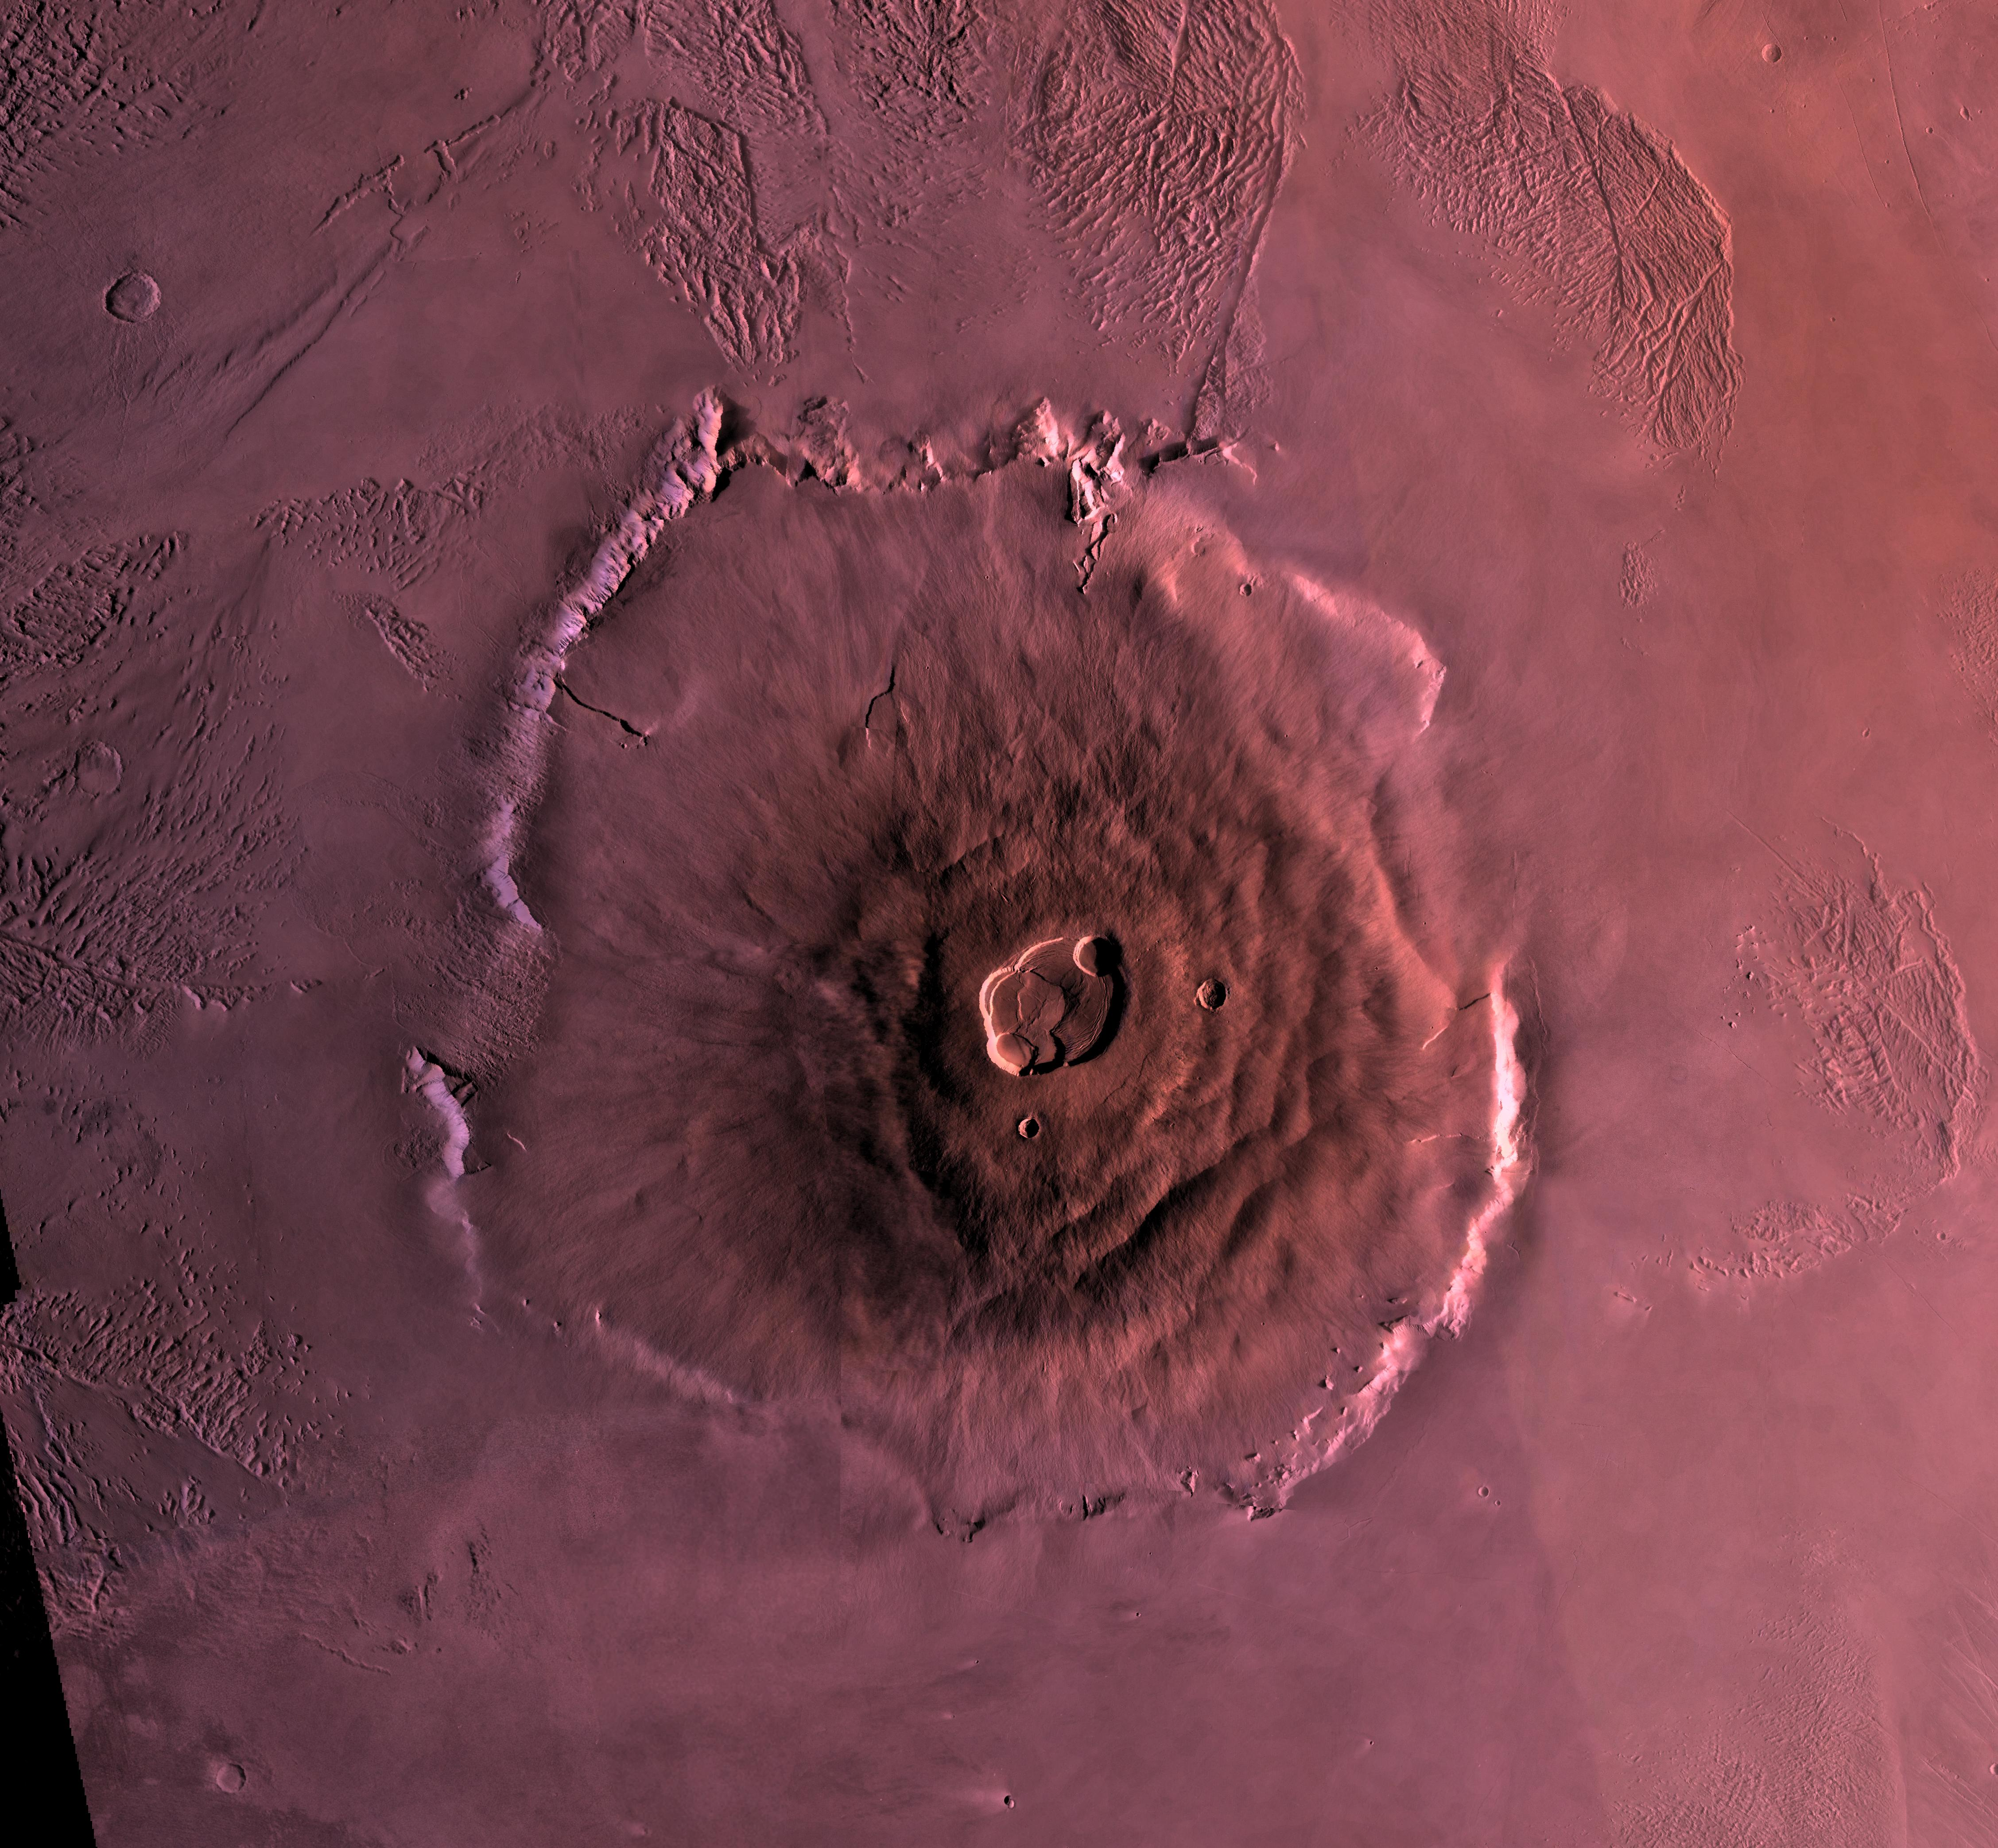
\includegraphics[width=0.95\paperwidth, height=0.80\paperheight, keepaspectratio]{olympus_mons}}\\
  {\footnotesize Olympus Mons, Mars: a shield volcano $\sim$600~km wide and $\sim$21~km high, with nested summit calderas. Viking Orbiter mosaic. Credit: NASA/JPL/USGS.}
\end{frame}

\begin{frame}{Why is Olympus Mons so large?}
  \begin{columns}[c]
    \column{\recapfigcolnarrow}
    \ipsrecapfig{olympus_mons_size_comparison}
    \source{Course figure}

    \column{\recaptextcolwide}
    Heights on one linear scale, widths schematic: Olympus Mons 21.2~km, Mauna Kea 10.2~km from the sea floor, Everest 8.8~km.
    \vskip8pt
    \keyresult{No plate motion: one plume feeds one edifice for billions of years. Lower gravity, $g \approx 0.38\,g_\oplus$, lets the crust hold a $\sim$2.6$\times$ taller pile.}
  \end{columns}
\end{frame}

% ── Lunar maria ───────────────────────────────────────────
\begin{frame}
  \centering
  \makebox[\linewidth][c]{\includegraphics[width=0.95\paperwidth, height=0.80\paperheight, keepaspectratio]{moon_nearside_annotated}}\\
  {\footnotesize The lunar maria: flood basalts that filled the nearside basins between 3.9 and 3.1~Ga and cover $\sim$16\% of the surface. LROC wide-angle mosaic. Credit: NASA/GSFC/Arizona State University.}
\end{frame}

% ── Volcanism comparison table ────────────────────────────
\begin{frame}{Volcanism across the solar system}
  \centering
  \footnotesize
  \begin{tabular}{l l l l}
    \toprule
    \textbf{Body} & \textbf{Style} & \textbf{Driving mechanism} & \textbf{Examples} \\
    \midrule
    Earth & Effusive + explosive & Internal heat + recycling & Hawaii, mid-ocean ridges \\
    Moon  & Flood basalts (extinct) & Residual heat (3.9--3.1~Ga) & Maria \\
    Mars  & Shield volcanoes & Mantle plumes, no plates & Olympus Mons, Tharsis \\
    Venus & Lava plains + shields & Internal heat, stagnant lid & Maat Mons \\
    Io    & Ultramafic flows & Tidal heating & Loki Patera, Pele \\
    \bottomrule
  \end{tabular}
  \vskip8pt
  Venus returns in Lecture~9, Io in Lecture~11.
\end{frame}


% ── Break ───────────────────────────────────────────────────
\breakslide


% ════════════════════════════════════════════════════════════
\sectionimage{san_andreas_aerial}{The San Andreas Fault across the Carrizo Plain, California. Credit: Ikluft, Wikimedia Commons, CC BY-SA 4.0}
\section{Tectonics}
% ════════════════════════════════════════════════════════════

% ── Plate tectonics ───────────────────────────────────────
\begin{frame}{Plate tectonics: Earth's unique regime}
  \begin{columns}[c]
    \column{\recapfigcol}
    \ipsrecapfig{plate_tectonics}
    \source{Wikimedia, CC BY-SA 3.0}

    \column{\recaptextcol}
    Earth is the \textbf{only} body with active plate tectonics:
    \begin{itemize}
      \item $\sim$15 rigid plates, moving at 1--10~cm\,yr$^{-1}$
      \item \textbf{Divergent:} ridges, new crust
      \item \textbf{Convergent:} subduction, recycling
      \item \textbf{Transform:} horizontal sliding
    \end{itemize}
    \vskip4pt
    Subduction closes the \textbf{carbonate-silicate cycle}.
  \end{columns}
\end{frame}

% ── Stagnant lid ──────────────────────────────────────────
\begin{frame}{Stagnant-lid convection}
  \begin{itemize}
    \item Every other terrestrial body: one rigid lithospheric lid
    \item The mantle convects beneath it; heat leaves by conduction and occasional volcanism
    \item The thick lid insulates: the mantle stays warm, but melt reaches the surface only through rare plumes (Tharsis), and volcanism fades as the lid grows
  \end{itemize}
  \vskip8pt
  \keyresult{Stagnant lid is the default for temperature-dependent viscosity. Breaking the lid, as Earth does, needs water weakening and self-sustaining damage.}
\end{frame}

% ── Valles Marineris ──────────────────────────────────────
\begin{frame}
  \centering
  \makebox[\linewidth][c]{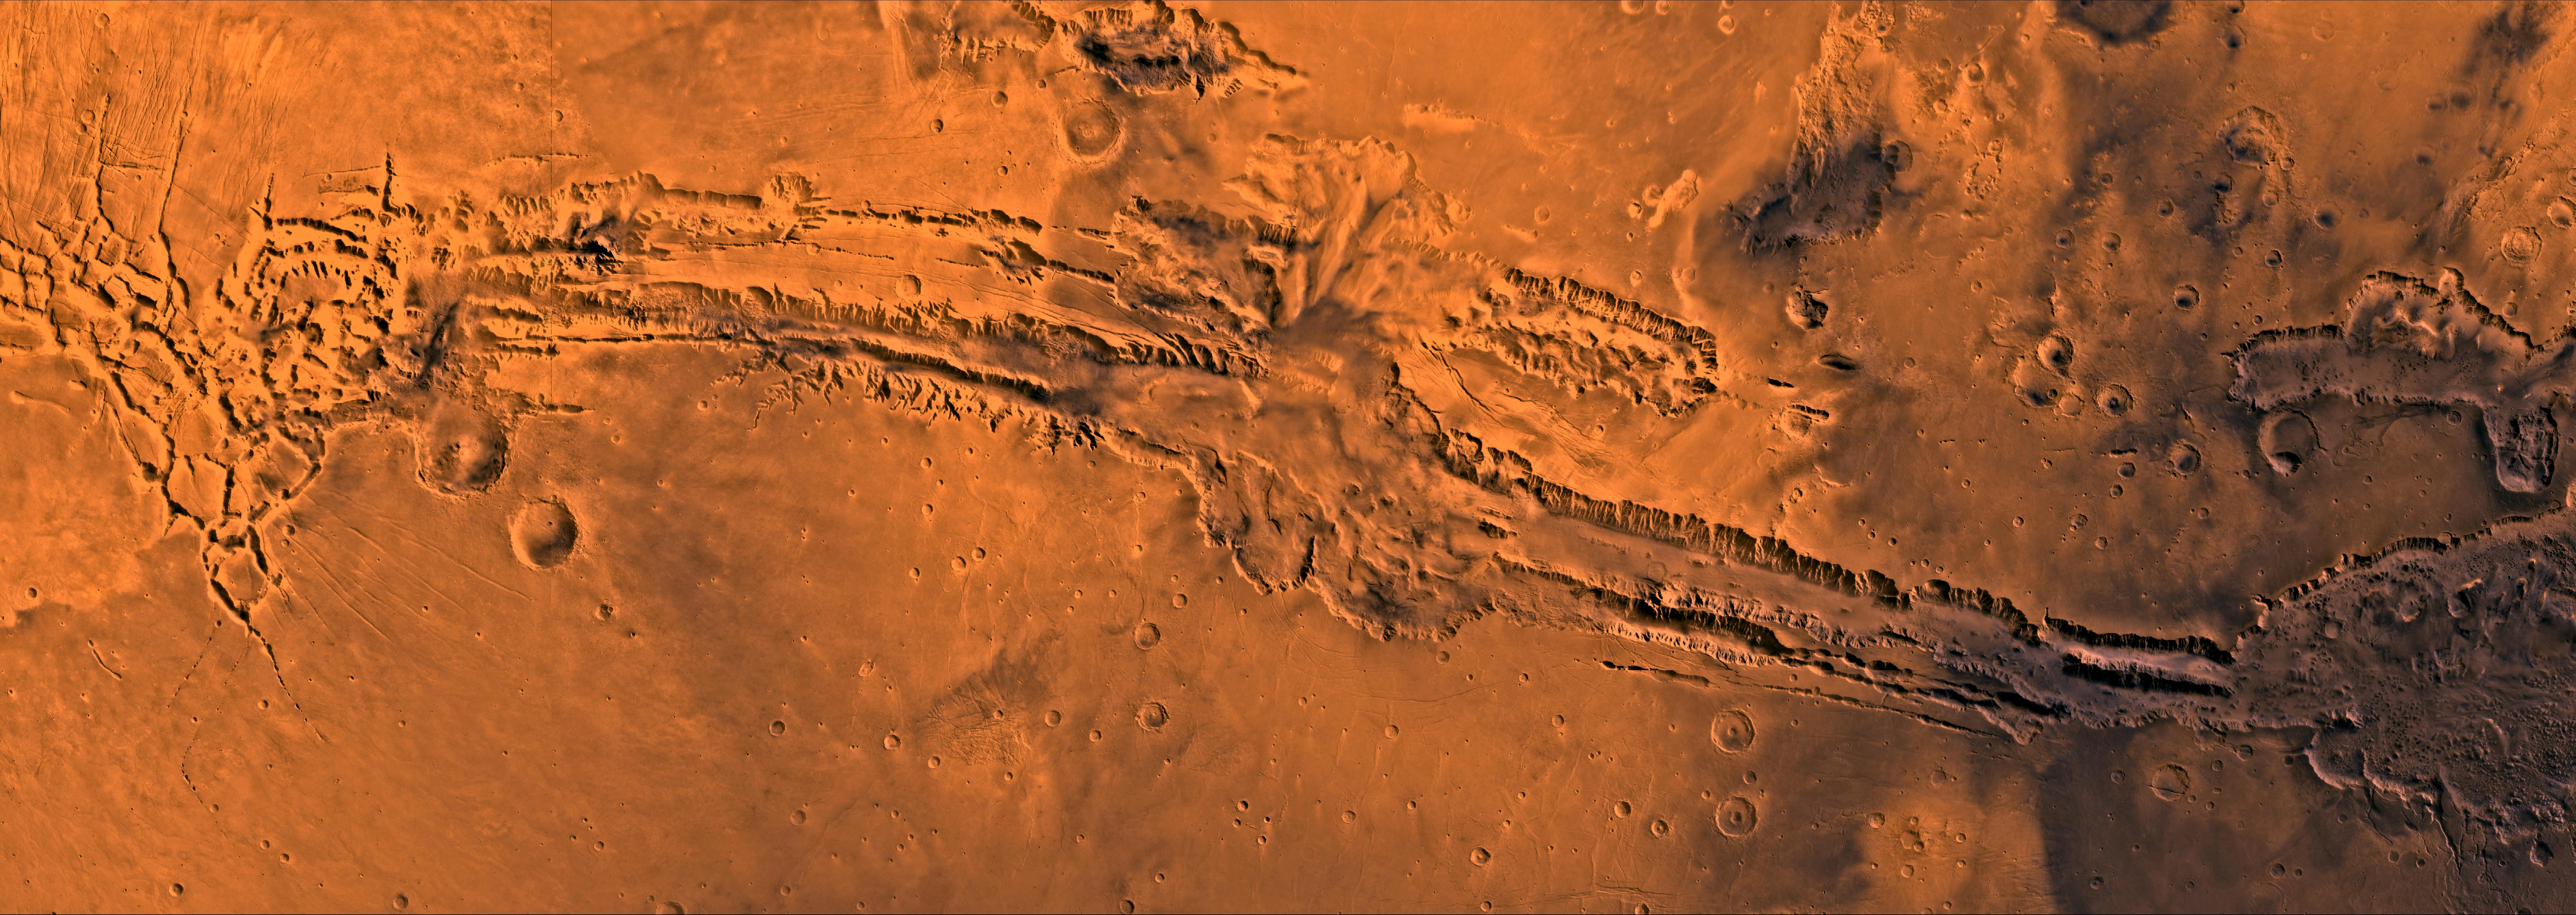
\includegraphics[width=0.95\paperwidth, height=0.80\paperheight, keepaspectratio]{valles_marineris}}\\
  {\footnotesize Valles Marineris in a Viking Orbiter mosaic: Noctis Labyrinthus on the left, then the Melas, Candor and Coprates chasmata, and the chaotic terrain feeding Chryse Planitia on the right. Credit: NASA/JPL/USGS.}
\end{frame}

\begin{frame}{Mars: Tharsis and Valles Marineris}
  \begin{columns}[c]
    \column{\recapfigcol}
    \ipsrecapfig{valles_marineris}
    \source{NASA/JPL/USGS}

    \column{\recaptextcol}
    \begin{itemize}
      \item \textbf{Tharsis:} volcanic plateau $\sim$5000~km wide, $\sim$10~km high, above a mantle plume
      \item \textbf{Valles Marineris:} $\sim$4000~km long, up to 7~km deep, rifted open by the Tharsis load
    \end{itemize}
    \vskip6pt
    \keyresult{No plate boundaries, yet the largest rift in the solar system. One volcanic load did what plate divergence does on Earth.}
  \end{columns}
\end{frame}

% ── Mars topography ───────────────────────────────────────
\begin{frame}{Mars topography: the hemispheric dichotomy}
  \centering
  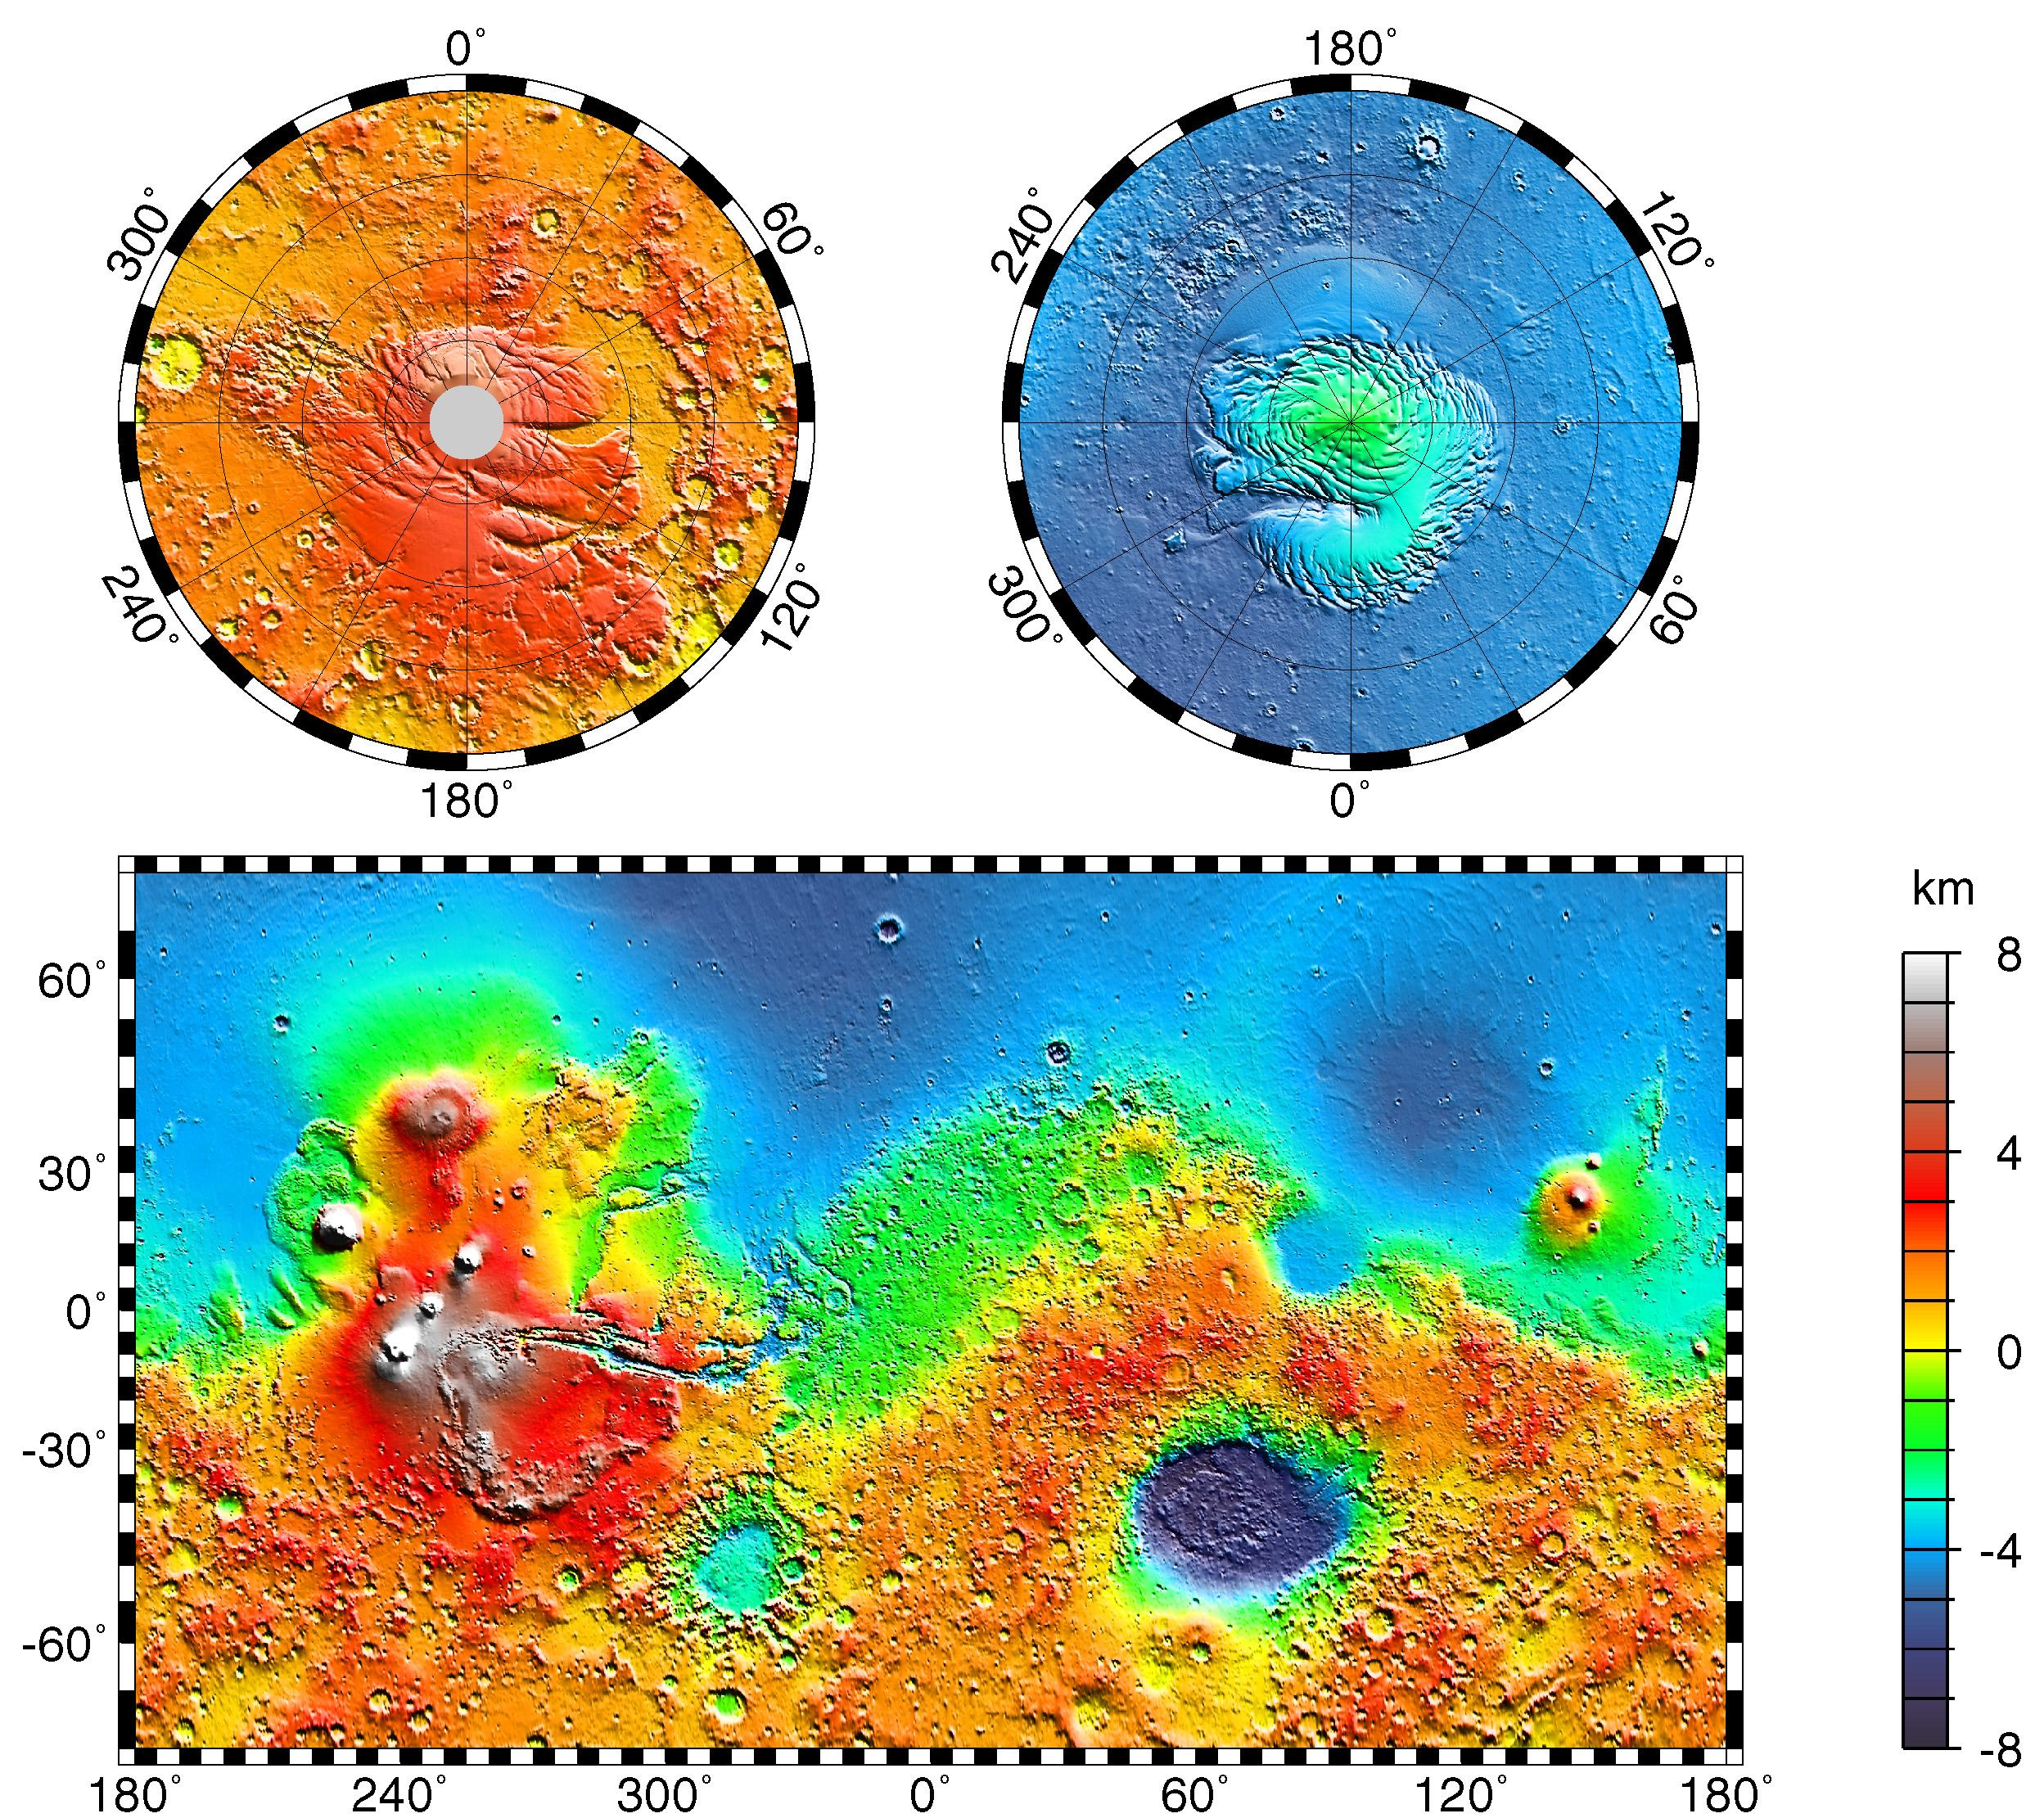
\includegraphics[width=\linewidth,height=0.62\textheight,keepaspectratio]{mars_topography}
  \source{NASA/JPL/GSFC/MOLA Science Team}
  \vskip4pt
  {\small $\sim$6~km between the southern highlands and the northern lowlands. Tharsis with 4 giant volcanoes; Hellas at $-$8.2~km; Valles Marineris at the equator.}
\end{frame}

% ── Mercury lobate scarp ──────────────────────────────────
\begin{frame}
  \centering
  \makebox[\linewidth][c]{\includegraphics[width=0.95\paperwidth, height=0.80\paperheight, keepaspectratio]{mercury_lobate_scarp}}\\
  {\footnotesize A lobate scarp on Mercury, a contraction thrust fault, imaged by MESSENGER. Credit: NASA/Johns Hopkins APL/Carnegie Institution of Washington.}
\end{frame}

\begin{frame}{Mercury: a planet that shrank}
  \begin{columns}[c]
    \column{\recapfigcolnarrow}
    \ipsrecapfig{mercury_lobate_scarp}
    \source{NASA/Johns Hopkins APL/Carnegie Institution of Washington}

    \column{\recaptextcolwide}
    \begin{itemize}
      \item The iron core cooled and solidified; the radius shrank by up to $\sim$7~km
      \item The crust took up the contraction on \textbf{lobate scarps}: thrust faults hundreds of km long, 1--3~km high
    \end{itemize}
    \vskip6pt
    \keyresult{The fault cuts craters, so the contraction is younger than they are. A cooling interior keeps deforming a stagnant lid.}
  \end{columns}
\end{frame}


% ════════════════════════════════════════════════════════════
\sectionimage{mars_dunes_bridges}{Barchan dunes in Nili Patera, Mars, imaged by HiRISE. Credit: NASA/JPL-Caltech/University of Arizona}
\section{Erosion and weathering}
% ════════════════════════════════════════════════════════════

% ── Dunes on Mars ─────────────────────────────────────────
\begin{frame}
  \centering
  \makebox[\linewidth][c]{\includegraphics[width=0.95\paperwidth, height=0.74\paperheight, keepaspectratio]{mars_dunes_bridges}}\\
  {\footnotesize Barchan dunes in Nili Patera, Mars. Repeat HiRISE images show whole dunes advancing at sand fluxes comparable to Earth's, under an atmosphere 170 times thinner (Bridges et al.\ 2012). Credit: NASA/JPL-Caltech/University of Arizona.}
\end{frame}

% ── Dunes on Titan ────────────────────────────────────────
\begin{frame}
  \centering
  \makebox[\linewidth][c]{\includegraphics[width=0.95\paperwidth, height=0.80\paperheight, keepaspectratio]{titan_dunes}}\\
  {\footnotesize Longitudinal dunes in Titan's Shangri-La region, Cassini SAR: organic sand, water-ice bedrock, the same aeolian physics. Credit: NASA/JPL-Caltech/ASI.}
\end{frame}

% ── Fluvial processes ─────────────────────────────────────
\begin{frame}{Fluvial (water) processes}
  \begin{columns}[c]
    \column{\recapfigcolnarrow}
    \ipsrecapfig{mars_valley_networks_viking}
    \source{NASA/JPL/USGS}

    \column{\recaptextcolwide}
    \raggedright
    \textbf{Mars valley networks:} Noachian ($>$3.7~Ga), dendritic, sustained liquid water
    \vskip6pt
    \textbf{Outflow channels:} hundreds of km long, catastrophic groundwater release
    \vskip6pt
    \textbf{Titan:} methane rivers; Huygens landed on rounded ice pebbles in a dry riverbed (2005)
  \end{columns}
\end{frame}

% ── Two kinds of Martian water feature ────────────────────
\begin{frame}
  \centering
  \makebox[\linewidth][c]{\includegraphics[width=0.95\paperwidth, height=0.80\paperheight, keepaspectratio]{mars_outflow_aram}}\\
  {\footnotesize A Martian outflow channel cutting through Aram Chaos. Credit: NASA/JPL-Caltech/MSSS.}
\end{frame}

\begin{frame}{Two kinds of water feature on Mars}
  \begin{columns}[c]
    \column{\recapfigcolnarrow}
    \ipsrecapfig{mars_outflow_aram}
    \source{NASA/JPL-Caltech/MSSS}

    \column{\recaptextcolwide}
    \begin{itemize}
      \item \textbf{Outflow channels} (here): braided islands, scoured troughs, one catastrophic flood
      \item \textbf{Valley networks}: dendritic, low discharge, long enough to need precipitation
    \end{itemize}
    \vskip6pt
    \keyresult{Read the shape, not just the presence of water. One says flood, the other says climate.}
  \end{columns}
\end{frame}

% ── Glacial and chemical weathering ───────────────────────
\begin{frame}{Glacial and chemical weathering}
  \begin{columns}[c]
    \column{\recapfigcolnarrow}
    \centering
    \includegraphics[width=\linewidth,height=0.31\textheight,keepaspectratio]{fedchenko_glacier}\\
    {\tiny\color{ipsText!60} Fedchenko Glacier, Pamir. Credit: NASA/ISS}\\[3pt]
    \includegraphics[width=\linewidth,height=0.31\textheight,keepaspectratio]{mars_clay_unit_glen_torridon}\\
    {\tiny\color{ipsText!60} Clay-bearing unit, Glen Torridon, Gale crater. Credit: NASA/JPL-Caltech/MSSS}

    \column{\recaptextcolwide}
    \textbf{Glacial:} ice flows under its own weight. Earth's ice sheets covered $\sim$30\% of land at the Last Glacial Maximum; Mars has polar caps and buried mid-latitude ice.
    \vskip8pt
    \textbf{Chemical:} silicate weathering is Earth's carbon sink. On Mars, clays, sulfates and carbonates seen from orbit record past liquid water.
  \end{columns}
\end{frame}


% ════════════════════════════════════════════════════════════
\sectionimage{venus_magellan}{Venus in Magellan radar, the surface seen through an opaque atmosphere. Credit: NASA/JPL}
\section{Remote sensing of surfaces}
% ════════════════════════════════════════════════════════════

% ── Four orbital techniques ───────────────────────────────
\begin{frame}{Four ways to see a surface from orbit}
  We land at a few sites. Almost all surface knowledge comes from orbit.
  \vskip8pt
  \begin{description}
    \item[Reflectance spectroscopy] minerals from absorption bands (CRISM at Mars: clays, carbonates)
    \item[Radar imaging] through clouds and haze (Magellan at Venus, Cassini at Titan)
    \item[Laser altimetry] topography to $\sim$1~m (MOLA made the Mars map you just saw)
    \item[Gravity field mapping] buried mass and crustal thickness (GRAIL at the Moon)
  \end{description}
\end{frame}

% ── GRAIL crustal thickness ───────────────────────────────
\begin{frame}
  \centering
  \makebox[\linewidth][c]{\includegraphics[width=0.95\paperwidth, height=0.80\paperheight, keepaspectratio]{grail_crustal_thickness}}\\
  {\footnotesize Lunar crustal thickness from GRAIL, nearside (left) and farside (right). Credit: NASA/MIT/GSFC/JPL-Caltech.}
\end{frame}

\begin{frame}{Weighing the lunar crust}
  \begin{columns}[c]
    \column{\recapfigcolnarrow}
    \ipsrecapfig{grail_crustal_thickness}
    \source{NASA/MIT/GSFC/JPL-Caltech}

    \column{\recaptextcolwide}
    \begin{itemize}
      \item Two satellites track their separation; gravity plus topography gives the crust-mantle depth
      \item Mean thickness $\sim$34--43~km; thin under the big basins, thick on the farside
    \end{itemize}
    \vskip6pt
    \keyresult{Gravity sees what images cannot: a basin is a hole punched through most of the crust.}
  \end{columns}
\end{frame}


% ════════════════════════════════════════════════════════════
\sectionimage{lunar_regolith_wide}{Apollo 11 bootprint in the lunar regolith. Credit: NASA}
\section{Regolith and space weathering}
% ════════════════════════════════════════════════════════════

% ── Impact gardening and nanophase iron ───────────────────
\begin{frame}{A shattered skin on every airless world}
  \begin{columns}[c]
    \column{\recapfigcolnarrow}
    \ipsrecapfig{lunar_regolith}
    \source{NASA/Apollo 11}

    \column{\recaptextcolwide}
    \textbf{Regolith:} loose debris made by impact gardening; 2--4~m on the maria, 6--8~m on the highlands
    \vskip8pt
    \textbf{Space weathering:} solar wind and micrometeorites make nanophase iron; surfaces turn \textbf{darker and redder}, so fresh craters like Tycho look bright
  \end{columns}
\end{frame}


% ════════════════════════════════════════════════════════════
\sectionimage{enceladus_cryovolcanism}{Enceladus plumes. Credit: NASA/JPL-Caltech/SSI}
\section{Cryovolcanism on icy bodies}
% ════════════════════════════════════════════════════════════

% ── Cryovolcanism overview ────────────────────────────────
\begin{frame}{Cryovolcanism: volcanism on ice worlds}
  \begin{itemize}
    \item The ``magma'' is water, ammonia-water or methane at 100--270~K; on Triton, nitrogen gas at $\sim$38~K
    \item \textbf{Tidal heating} keeps oceans liquid under the ice shells
    \item Enceladus erupts water plumes, Europa resurfaces, Triton vents nitrogen
  \end{itemize}
  \vskip8pt
  \keyresult{Liquid water far outside the habitable zone, kept by tides, not sunlight. The bodies return in Lecture~11.}
\end{frame}

% ── Europa lineae and chaos ───────────────────────────────
\begin{frame}
  \centering
  \makebox[\linewidth][c]{\includegraphics[width=0.95\paperwidth, height=0.74\paperheight, keepaspectratio]{europa_chaos}}\\
  {\footnotesize Double ridges and lineae near Pwyll crater on Europa, Galileo SSI. So few craters that the surface is only 40--90~Myr old. Credit: NASA/JPL-Caltech/University of Arizona/University of Colorado.}
\end{frame}


% ════════════════════════════════════════════════════════════
\sectionimage{io_nusku_change}{A new eruption on Io, JunoCam 2024. Credit: NASA/JPL-Caltech/SwRI/MSSS/Jason Perry}
\section{Recent advances}
% ════════════════════════════════════════════════════════════

% ── Io monitoring ─────────────────────────────────────────
\begin{frame}
  \centering
  \makebox[\linewidth][c]{\includegraphics[width=0.95\paperwidth, height=0.80\paperheight, keepaspectratio]{io_nusku_change}}\\
  {\footnotesize The Nusku region on Io two months apart in 2024, JunoCam. Credit: NASA/JPL-Caltech/SwRI/MSSS/Jason Perry.}
\end{frame}

\begin{frame}{Catching an eruption in the act on Io}
  \begin{columns}[c]
    \column{\recapfigcolnarrow}
    \ipsrecapfig{io_nusku_change}
    \source{NASA/JPL-Caltech/SwRI/MSSS/Jason Perry}

    \column{\recaptextcolwide}
    \begin{itemize}
      \item February 2024: nothing unusual around the vent
      \item April 2024: a red ring of fresh sulfur-rich pyroclastic deposits
    \end{itemize}
    \vskip6pt
    \keyresult{Io is the one body beyond Earth where volcanic resurfacing shows up between two flybys. Juno gives the first sustained monitoring since Galileo.}
  \end{columns}
\end{frame}

% ── Summary ────────────────────────────────────────────────
\begin{frame}{Summary}
  \begin{enumerate}
    \item Surfaces record \textbf{endogenic} (volcanism, tectonics) against \textbf{exogenic} (impacts, erosion) processes
    \item Crater scaling law: $D \sim (E/\rho g)^{1/4}$, a fourth root of the energy
    \item Crater counting plus Apollo calibration gives absolute surface ages
    \item No plate tectonics: giant volcanoes, one rift, a shrinking Mercury; Earth alone breaks its lid
    \item Fluvial features on Mars are strong evidence for past liquid water
  \end{enumerate}
  \vskip8pt
  \textbf{Next:} Lecture~8 goes underneath, to the interiors that drive the endogenic half of this record.
\end{frame}

% ── Final slide ─────────────────────────────────────────────
\begin{frame}[plain,noframenumbering]
  \begin{tikzpicture}[remember picture, overlay]
    \ipscontain{title_background}
    \fill[ipsPrimary, opacity=0.70] (current page.north west) rectangle (current page.south east);
  \end{tikzpicture}
  \vfill
  \begin{center}
    {\color{white}\Large\bfseries Questions?}
    \vskip20pt
    {\color{white!85}\large Next: Lecture 8, Planetary interiors: structure, composition \& dynamics}\\[4pt]
    {\color{white!85}\small Thu 1 Oct, 11:00--13:00, room 5419.0161 (Collegezaal)}\\[12pt]
    {\color{white!85}\small Next tutorial: Fri 2 Oct, 13:00--15:00, room 5419.0161 (Collegezaal)}\\[20pt]
    {\color{white!70}\small \texttt{https://ips.formingworlds.space}}
  \end{center}
  \vfill
\end{frame}

\end{document}
